\begin{frame}[t]{Trabajando con un repositorio}
    \begin{comando}
        git clone
    \end{comando}

    \begin{block}{}
        Para obtener una \textbf{copia local} de un repositorio existente en algún servidor,
        utilizamos el comando \texttt{git clone [URL]}.
    \end{block}
    \begin{block}{}
        Importante: \textit{git clone [URL]} crea un nuevo directorio con el
        repositorio clonado. Debemos hacer \textit{cd <repo>} luego de clonarlo!
    \end{block}

    \pause
    \begin{ejercicio}{Ejercicio}
        Clonen el repositorio de prueba para el taller. Para eso pueden ejecutar \texttt{git clone https://git.cubawiki.com.ar/mlang/ejemplo}.
        Después ejecuten \texttt{cd ejemplo} para situarse en el repositorio recién clonado.
    \end{ejercicio}
\end{frame}

\begin{frame}{¿Directorio o repositorio?}
    \begin{figure}
    \centering
    \begin{minipage}{0.45\textwidth}
        \centering        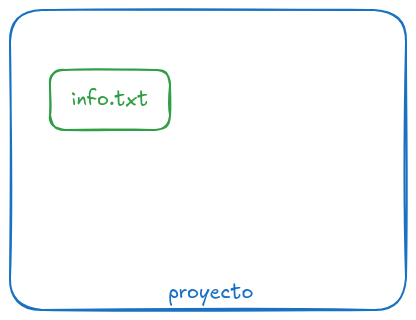
\includegraphics[width=0.95\textwidth]{graficos/carpeta.png} 
        \caption{Directorio 'proyecto' \textbf{antes} de hacer \textit{git init}}
    \end{minipage}\hfill
    \begin{minipage}{0.45\textwidth}
        \centering        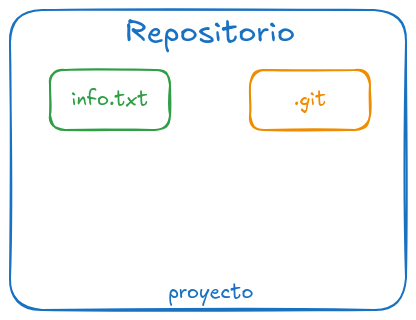
\includegraphics[width=0.95\textwidth]{graficos/Repo.png} 
        \caption{Directorio 'proyecto' \textbf{luego} de hacer \textit{git init}}
    \end{minipage}
\end{figure}

    
\end{frame}

\begin{frame}[fragile, t]{¿Está preparado, confirmado o ninguna de las dos?}
    \begin{comando}
        git status
    \end{comando}
        \begin{block}{Output de ejemplo}
            \begin{center}
            \texttt{nothing to commit (create/copy files and use "git add" to track)}
            \end{center}
        \end{block}
    \pause
    \begin{ejercicio}{Ejercicio}
        Crear un nuevo archivo en nuestro repositorio y ejecuten \textit{git status}. Vean como cambia el mensaje. Recuerden el comando \textit{touch}.
    \end{ejercicio}

\end{frame}
\begin{frame}[fragile, t]{¿Está preparado, confirmado o ninguna de las dos?}
    \begin{comando}
        git status
    \end{comando}
    \begin{block}{Output de ejemplo}
            \begin{center}
            \texttt{Untracked files:
  (use "git add <file>..." to include in what will be committed) \\archivo}
            \end{center}
        \end{block}
\begin{ejercicio}{Ejercicio}
    Ejecuten el comando que les sugiere \textit{git} para incluír el archivo que crearon recién. Hagan \textit{git status}.
\end{ejercicio}
\end{frame}


\begin{frame}{¿Está preparado, confirmado o ninguna de las dos?}
    \begin{figure}
    \centering
    \begin{minipage}{0.45\textwidth}
        \centering        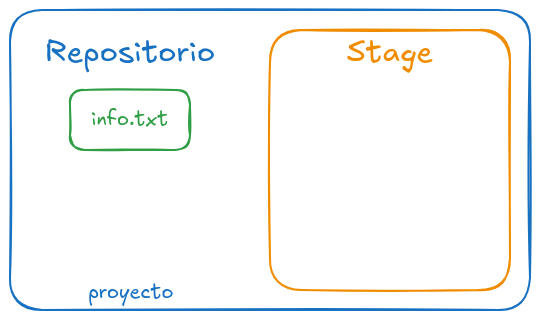
\includegraphics[width=0.95\textwidth]{graficos/stage_1.png} 
        \caption{Directorio 'proyecto' \textbf{antes} de hacer \textit{git add info.txt}}
    \end{minipage}\hfill
    \begin{minipage}{0.45\textwidth}
        \centering        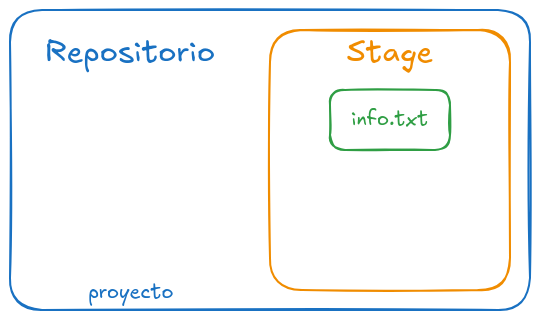
\includegraphics[width=0.95\textwidth]{graficos/stage_2.png} 
        \caption{Directorio 'proyecto' \textbf{luego} de hacer \textit{git add info.txt}}
    \end{minipage}
\end{figure}
\end{frame}

\begin{frame}[fragile, t]{¿Está preparado, confirmado o ninguna de las dos?}
    \begin{comando}
        git status
    \end{comando}
    \begin{block}{Output de ejemplo}
            \begin{center}
            \texttt{Changes to be committed:
  (use "git rm --cached <file>..." to unstage)
        \\new file:  archivo}
            \end{center}
        \end{block}
   \begin{block}{}
       Con esto vemos que \textit{git} ahora conoce al nuevo archivo, y lo va a tener en cuenta cuando hagamos un \textit{commit} proximamente.
   \end{block}     

   \pause
\end{frame}

% es como un checkpoint
\begin{frame}[t]{Confirmando cambios}
    \begin{comando}
        git commit
    \end{comando}

    \pause
    \begin{block}{}
        Una vez que tenemos ciertos cambios marcados con \textit{add}, podemos confirmarlos
        ejecutando \texttt{git commit -m "mensaje"}.

        \vspace{0.5em}

        Donde \texttt{[mensaje]} es una breve descripción de los cambios que acabamos de confirmar.
    \end{block}
    \pause
    \begin{resumen}{¡Yo elijo lo que pongo en el stage!}
        \begin{itemize}
            \item Puedo poner y sacar archivos como \textit{staged} usando \texttt{git add} y \texttt{git rm --cached}.
            \item Git nos sugiere estos comandos luego de hacer \textit{git status}.
        \end{itemize}    
    \end{resumen}
    \pause
    \begin{ejercicio}{Ejercicio}
        Hagan el \textit{commit} que venían preparando y elijan un mensaje. Luego hagan \textit{git status}.
    \end{ejercicio}
\end{frame}

\begin{frame}{¿Está preparado, confirmado o ninguna de las dos?}
    \begin{figure}
    \centering
    \begin{minipage}{0.45\textwidth}
        \centering        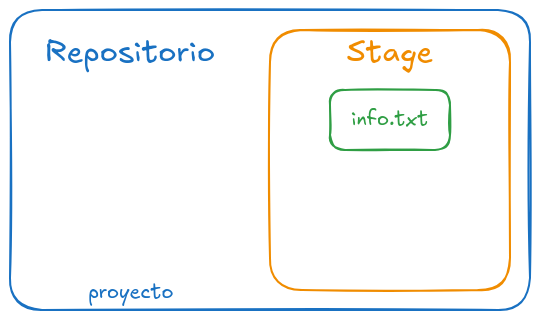
\includegraphics[width=0.95\textwidth]{graficos/stage_2.png} 
        \caption{Directorio 'proyecto' \textbf{antes} de hacer \textit{commit}}
    \end{minipage}\hfill
    \begin{minipage}{0.45\textwidth}
        \centering        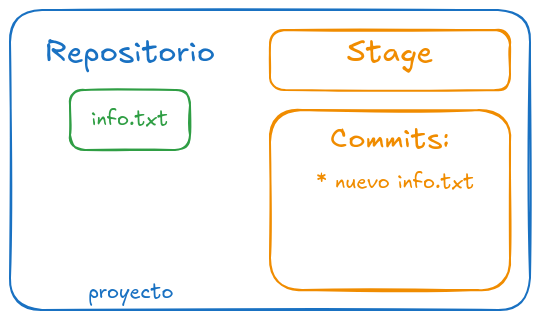
\includegraphics[width=0.95\textwidth]{graficos/commit.png} 
        \caption{Directorio 'proyecto' \textbf{luego} de hacer \textit{git commit -m "nuevo info.txt"}}
    \end{minipage}
\end{figure}
\end{frame}

\begin{frame}{¿Y si modifico el archivo luego del commit?}
    \begin{comando}
        git status
    \end{comando}
    \begin{block}{Output de ejemplo}
    \centering
        \texttt{Changes not staged for commit:\\
  (use "git add <file>..." to update what will be committed)\\
  (use "git restore <file>..." to discard changes in working directory)\\
	modified:   archivo}
    \end{block}  
\end{frame}

\begin{frame}{Estados de un archivo}

    \begin{block}{Los cuatro estados de los archivos}
            \begin{enumerate}
    \item Untracked = Sin seguimiento
    \item Unmodified = Sin modificar
    \item Modified = Modificado
    \item Staged, to be commited = Confirmado
    \end{enumerate}
    \end{block}
    \begin{center}
        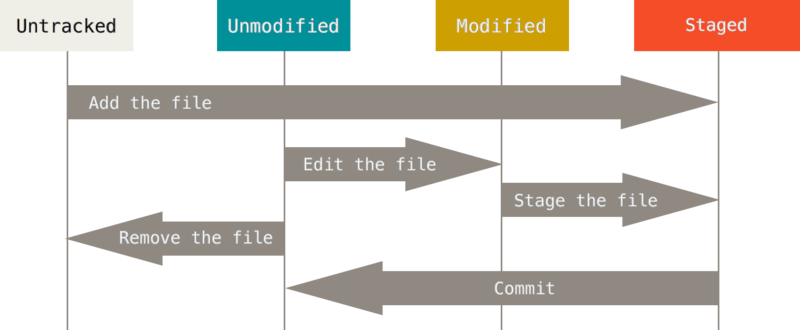
\includegraphics[width=4in]{images/lifecycle.png}
    \end{center}    
\end{frame}

% \begin{frame}[t]{¿Cómo funciona Git?}
%     \begin{center}
%         \begin{block}{Sistema de \textit{Snapshots}}
%         \begin{enumerate}
%             \item Piensa a los archivos como una serie de 'fotos'.
%             \item Con cada commit, es decir, cada vez que guardas el estado del repo, saca una 'foto' del \textit{stage} y guarda una referencia a esa foto.
%             \item Para saber el contenido de un archivo, git mira todos los commits que lo incluyan.
            
%         \end{enumerate}

%         \end{block}

%         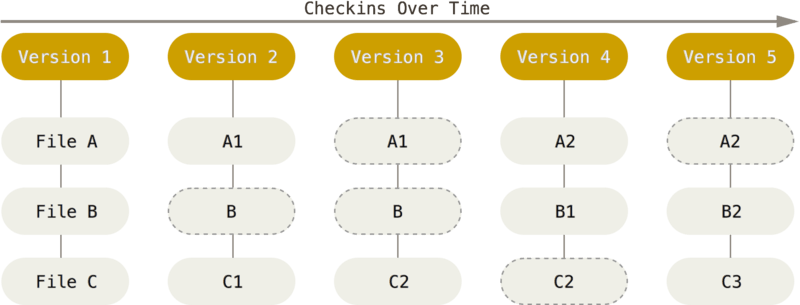
\includegraphics[width=4in]{images/snapshots.png}
%     \end{center}
    
% \end{frame}

\begin{frame}{Historial}
 \begin{comando}
     git log
 \end{comando}
 \pause
 \begin{block}{}
     Este comando nos sirve para ver el historial de cambios, o commits. Además nos dice quién hizo cada cosa, cuándo, y su correo electrónico.
 \end{block}
 \pause
    \begin{figure}[ht]
        \begin{center}
            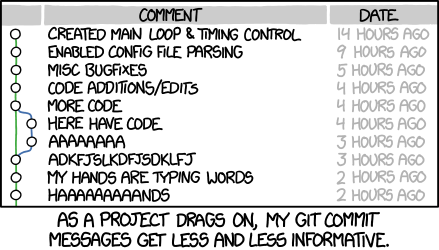
\includegraphics[height=1.7in]{images/xkcd-git-commit.png}
        \end{center}
        \caption{Fuente: \url{https://xkcd.com/1296/}}
    \end{figure}
\end{frame}

% \begin{frame}{Integrando los conceptos}
% \begin{ejercicio} {Ejercicio integrador}
%     \begin{enumerate}
%         \item En el repositorio donde venían trabajando, creen dos archivos 'pepe' y 'juan'. Recuerden el comando \textit{touch}.
%         \pause
%         \item Hagan add y commit con un mensaje como 'creación de archivos'.
%         \pause
%         \item Usando nano, escriban unas palabras acerca de pepe y juan, en sus archivos respectivos.
%         \pause
%         \item 
%         \pause
%         \item Para ver el estado final de su repo con un gráfico,\\
%         hagan \textit{git log - -graph}
%     \end{enumerate}
% \end{ejercicio}
%\end{frame}

